\subsubsection{Zależność między Zigbee a 802.15.4}


Podstawowym podejściem służącym do ustabilizowania złożonych rozwiązań technologicznych jest podział na autonomiczne moduły-warstwy. Podejście to jest szeroko stosowane w protokołach sieciowych gdzie spotykamy wielowarstwowe modele sieci z których każda warstwa jest odpowiedzialna za pewne z góry określone funkcję w sieci. Dane mogą być przesyłane z jednego poziomu do wyższej lub niższej warstwy.

Protokół ZigBee bazuje na dobrze znanym modelu OSI (Open System Interconnect). Podział Zigbee na warstwy przynosi wiele korzyści, z których główną jest możliwość modyfikacji lub nawet zamiany całej warstwy w wyniku ewolucji technologicznej co w przypadku monolitycznych rozwiązań wiąże się z refaktoryzacją całego protokołu.

\par Historia Zigbee: \\ \\

Nazwa ZigBee: stanowi nawiązanie do "tańca pszczół" czyli regularnych cyklicznych ruchów za pomocą których pszczoły informuują inne robotnice o wykonywanym zajęciu \\ 
\tab 	Historia powstania ZigBee sięga jeszcze ostatnich lat 20 wieku, kiedy to odbyło się wiele dyskusji w kręgach inżynierskich nad zastosowaniem komunikacji bezprzewodowej opartej na obecnych wtedy na rynku rozwiązań bazujących na WiFi lub bluetooth-u. Pierwszym kompletnym standardem który powstał w 2003 roku był IEEE 802.15.4 \\


\par Warstwowa budowa protokołu ZigBee \\ \\

\tab 	Standard IEEE 802.15.4 jest standardem dla warstwy fizycznej oraz dostępu do medium komunikacyjnego dla sieci LR-WPAN (low rate wireless personal area networks) .  Skupia się on na podstawowych najniższych warstwach komunikacji. Architektura protokołu bazuje na modelu OSI, jednakże tylko najniższe warstwy są ściśle ustandaryzowane mechanizmami takimi jak np. CSMA. Do interakcji z górnymi warstwami można użyć zalecanej normy IEEE 802.2 który określa logiczną podwarstwę sterowania dostępem do warstw wyższych z warstwy MAC poprzez warstwy pośrednie.
	\\
	Koncepcyjną budowę warstwową protokołu ZigBee przedstawia poniższy schemat:
	\\
	\\
\centerline{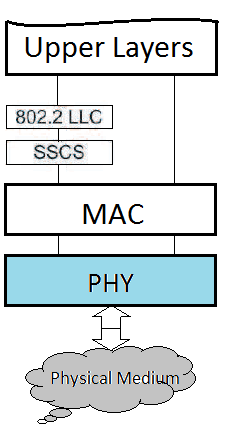
\includegraphics[scale=0.5]{./img/img_1__2_1_3}}
\\

\par Fizyczna warstwa ZigBee: \\ \\ 
\tab 	ZigBee jest standardem komunikacji radiowej. W swoich założeniach zaleca komunikację na częśtotliwościach 2.4 GHz (stosowane na całym świecie) oraz ze względu na panujące prawo determinujące komumikację radiową: dodatkowe pasmo na częstotliwości 915 MHz dla Ameryki i Australii oraz 868 MHz dla Europy.
\\
\tab 	Pasmo 2.4 GHz umożliwia transmisję o prędkości maksymalnej do 250Kbps oraz udostępnia 16 różnych kanałów transmisyjnych. 915 MHz (w rzeczywistości 902–928MHz) daje możliwość rozwinięcia prędkości 40Kbps i udostępnia 10 kanałów transmisyjnych, natomiast 868 MHz daje możliwość transmisji do 20Kbps i 1 kanał transmisyjny.
\\
	Standard ZigBee opierający się o normę 802.15.4 definiuje szeref mechanizmów zapewniających niezawodność transmisji danych. W warstwie fizycznej, dla częstotliwości 868/915 MHz jest wykorzystywane kodowanie "Binary Phase Shift Keying" czyli modulacji cyfrowej polegającej na kluczowaniu fazy, natomiast dla 2.4GHz transmisja wykorzystuje inną odmianę modulacji fazy O-QPSK. Są to proste szybkie metody modulacji które sprawdzają się dobrze w środowiskach o niskim stosunku SNR. \\

\par Warstwa MAC i mechanizmy wchodzące w skład warstwy MAC \\ \\
\tab 	CSMA jest mechanizmem definiowanym przez standard IEEEumożliwiającym urządzenią współdzielenie tego samego kanału transmisyjnego, zapobiegającemu występowaniu kolizji. Technika ta pochodzi z przed lat a jej mechanizm był wykorzystywany w sieciach Ethernetowych, dzięki czemu urządzenia nie potrzebowały się synchronizować między sobą. Metoda wielodostępu do tego samego kanału jest bardzo prosta i intuicyjna, opiera się na zasadzie "listen before you talk". Czyli każde urządzenie przed rozpoczęciem nadawania nasłuchuje na danym kanale i jeśli jest obecnie wolny nadaje wiadomość, w przeciwnym wypadku odczekuje okres czasu zależny od platformy i powtarza czynność dopóki kanał się nie zwolni, lub odczekiwany okres czasu przekroczy założony interwał i zgłosi błąd transmisji.
\\
\tab 	Mechanizm potwierdzania/ponawiania transmisji służy w sytuacji kiedy wiadomość zostanie poprawnie nadana jednak odbiorca nie będzie w stanie jej dobrze odebrać (np w sytuacji kiedy nie zgadza się suma kontrolna, lub rozmiar ramki). Każde urządzenie w momencie odebrania wiadomości ma krótki czas w którym musi wysłać potwierdzenie odbioru nazywane dalej ACK. Jeśli nadawca nie dostanie zgłoszenia ACK, przyjmuje on że z jakiś powodów wiadomość nie dotarła do odbiorcy i ponownie wysyła tę samą ramkę danych, ponownie czekając na potwierdzenie od odbiorcy. Proces ten jest powtarzany dopóki odpowiedź ACK nie zostanie odebrane lub nadawca przekroczy zdefiniowany przez siebie czas i zgłosi niedosłanie wiadomości.
\\	
\tab 	IEE 802.15.4 określa specyfikacje dotyczące PHY i sposobu adresowania za pomocą numerów MAC, dostarczając gotowe topologie dostosowane do systemów o różnym zastosowaniu poczynając od prostych architektór takich jak peer-to-peer czy star (gwiazda) a kończąc na takich jak mesh (nie skorelowane równoważne węzły) i cluster tree (architektura składająca się z połączonych drzew rozpiętych na blokach odbiorników). W zależności od architektury i zastosowania stosuje się systemy routingu które zaprojektowane głównie w celu zapewnienia ochrony energii spełniają również takie funkcje jak zapewnienie niskiej latencji dla transmitowanych danych, niezawodność transmisji oraz w ujęciu calościowym dla sieci odporność na uszkodzenia, niezawodność i elastyczność. 
\\

\par ZigBee rooting layer\\ \\
\tab 	Komponenty wchodzące w skład sieci: \\
\tab		Sieci ZigBee zawierają wiele  komponentów składowych. Podstawą jest urządzenie z którym chcemy się komunikować. Może być nim każdy układ elektroniczny np: sensor, interfejs graficzny urządzenie wejścia/wyjścia. Urządzenie to może być nazwane mianem FFD (full-function device) lub RFD (reduced-function device). Aby sieć miała sens funkcjonalny musi zawierac conajmniej jedno urządzenie FFD które stanie się koordynatorem sieci (w literaturze PAN (personal network area) coordinator). Dzięki koordynatorowi informacje zebrane z sieci mogą być przesłane dalej lub przetwarzane na miejscu.
\\
\tab		Urządzenie FFD może pracować w 3 trybach: jako PAN coordinator, coordinator lub zwykłe urządzenie, natomiast urządzenia typu RFD są przewidziane do prostych zastosowań nie wymagających wysyłania dużej ilości danych. Urządzenie FFD może prowadzić komunikację z jednym lub wieloma urządzeniami RFD jednocześnie natomiast RFD może prowadzić komunikację jedynie z 1 FFD.
\\		
\begin{center}
Literaturowe topologie sieci: \\
\end{center}

\par 
Star Topology (Topologia gwiazdy):\\ \\
\tab 	W topologii gwiazdy komunikacja jest nawiązana pomiędzy urządzeniami należącymi do sieci oraz pojedyńczą centralną jednostką kontrolera PAN coordinator. W analizie sieci przyjmuje się że PAN może być zasilany sieciowo natomiast urządzenia stanowiące wierzchołki gwiazdy są zasilane bateryjnie. \\
\tab 	Konfiguracja sieci rozpoczyna się od aktywacji pierwszego urządzenia FFD które może zostać koordynatorem sieci. Urządzenia mogą wybrać czy dany FFD może zostać  PAN coordinator-em sieci. Każde uruchomienie sieci powoduje na nowo wybór koordynatora sieci lub jego identyfikacje i sprawdzenie czy nie należy on już do innej sieci. Dzięki temu sieci o topologii gwiaździstej mogą pracować niezależnie od reszty otoczenia sieciowego.\\

\par 
Topologia Peer-to-peer:\\ \\
\tab		W topologii peer-to-peer podobnie jak w topologii gwiazdy mamy do czynienia z jednym urządzeniem pełniącym funkcję PAN coordinator, natomiast w porównaniu do topologii gwiazdy urządzenia mają swobodę komunikacji i mogą wymieniać ramki danych z każdym innym a nie tylko z koordynatorem. Sieci peer-to-peer dzięki swobodzie w komunikacji mogą być typu ad-hoc, self-organizing lub self-healing. Dzięki wielostopniowemu rutingowi sieci te zyskuja bardzo dużo na niezawodności.\\
\par
Topologia Cluster-tree:\\ \\
\tab		Sieci typu Cluster-tree są specjalnym przypadkiem w którym mamy doczynienia z kilkoma sieciamy typu peer-to-peer których koordynatorzy porozumiewają się między sobą na zewnątrz podsieci. Każda z podsieci staje się wtedy częścią nowego dużego drzewa. Po uruchomieniu sieci ze wszystkich koordynatorów tworzących podsieci jest wyłaniany jeden główny PAN coordinator, natomiast wszyscy inni lokalni koordynatorzy mogą swobodnie w swoich sieciach prowadzić takie operacje jak synchronizacja transmisja czy renegocjacje między urządzeniami. Po wyborze PAN coordinatora staje się on główną częścią klastra z CID (cluster ID) równym zero, następnie rozsyła on i przydziela identyfikatory swoim sąsiadą. Jeśli zdecyduja się oni dołączyć do sieci rozdają kolejne wolne CID-y swoim sąsiadą, dzięki czemu w sieciach lokalnych może następować komunikacja jak to miało miejsce w sieciach peer-to-peer natomiast jednocześnie wszystkie urządzenia są dostępną dla siebie częścią klastra.\\

\clearpage 